\documentclass{article}
\usepackage[margin=1in]{geometry}
\usepackage{xcolor}
\usepackage{graphicx}
\usepackage{tikz}
\usetikzlibrary{patterns, shadings}

% Try loading transparency library, but fallback if not available (older tikz)
\IfFileExists{tikzlibrarytransparency.code.tex}{\usetikzlibrary{transparency}}{}

\begin{document}

\section*{TeXpresso Render Commands Test}

\subsection*{Text and Fonts}
This is normal text. \\
\textbf{This is bold text.} \\
\textit{This is italic text.} \\
\textsf{This is sans-serif text.} \\
\texttt{This is typewriter text.} \\
\textsc{This is Small Caps text.}

\subsection*{Stroked Text (Outline)}
% XeTeX/Tectonic specific special for text render mode: 1 Tr = stroke
\special{pdf:literal 1 Tr 0.5 w}This is Stroked Text\special{pdf:literal 0 Tr}

\subsection*{Colors}
\textcolor{red}{Red Text} \\
\textcolor{green}{Green Text} \\
\textcolor{blue}{Blue Text} \\
\textcolor{cyan}{Cyan Text} \\
\textcolor{magenta}{Magenta Text} \\
\textcolor{yellow}{Yellow Text}

\newpage

\section*{Paths and Graphics (TikZ)}

\subsection*{Fill and Stroke}

\begin{tikzpicture}
    \draw[thick] (0,0) -- (2,0) -- (1,1.732) -- cycle;
    \node at (1,-0.5) {Stroked Triangle};
\end{tikzpicture}
\hfill

\begin{tikzpicture}
    \fill[orange] (0,0) circle (1cm);
    \node at (0,-1.5) {Filled Circle};
\end{tikzpicture}
\hfill

\begin{tikzpicture}
    \filldraw[fill=blue!20, draw=blue, thick] (0,0) rectangle (2,2);
    \node at (1,-0.5) {Filled \& Stroked Rect};
\end{tikzpicture}

\subsection*{Clipping}

\begin{tikzpicture}
    \draw[help lines] (0,0) grid (3,3);
    \clip (1.5,1.5) circle (1cm);
    \fill[red] (0,0) rectangle (3,3);
    \node[white] at (1.5,1.5) {Clipped};
\end{tikzpicture}

\subsection*{Shading (Gradients)}

\begin{tikzpicture}
    \shade[left color=red, right color=blue] (0,0) rectangle (4,1);
    \node at (2,-0.5) {Linear Gradient};
\end{tikzpicture}


\begin{tikzpicture}
    \shade[inner color=yellow, outer color=red] (0,0) circle (1cm);
    \node at (0,-1.5) {Radial Gradient};
\end{tikzpicture}

\newpage

\section*{Images, Transparency, and Patterns}

\subsection*{Images}
% Check if image exists, otherwise skipping to avoid error during blind compile
\IfFileExists{../doc/texpresso_logo_v2.png}{
    
\includegraphics[width=5cm]{../doc/texpresso_logo_v2.png}
}{
    \textbf{Image not found: ../doc/texpresso_logo_v2.png}
}

\subsection*{Transparency}
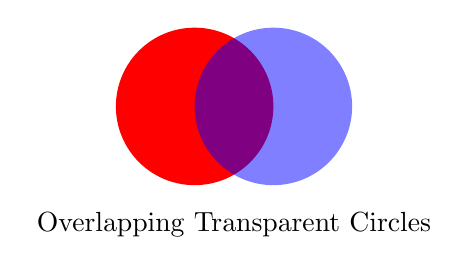
\begin{tikzpicture}
    \fill[red] (0,0) circle (1cm);
    \fill[blue, opacity=0.5] (1,0) circle (1cm);
    \node at (0.5,-1.5) {Overlapping Transparent Circles};
\end{tikzpicture}

% Group transparency if library loaded
\ifdefined\tikz@library@transparency@loaded

\begin{tikzpicture}
    \begin{scope}[transparency group]
        \fill[red] (0,0) rectangle (2,2);
        \fill[green] (1,1) rectangle (3,3);
    \end{scope}
    \node at (1.5,-0.5) {Transparency Group};
\end{tikzpicture}
\fi

\subsection*{Patterns}

\begin{tikzpicture}
    \fill[pattern=north east lines] (0,0) rectangle (2,2);
    \node at (1,-0.5) {Hatch Pattern};
\end{tikzpicture}
\hfill

\begin{tikzpicture}
    \fill[pattern=dots, pattern color=blue] (0,0) circle (1cm);
    \node at (0,-1.5) {Dots Pattern};
\end{tikzpicture}

\end{document}
